\section{Post-Processing}
\label{sec:exp-postproc}
    \twN{can phrase this more as a constrained optimisation problem with rejection percentages as bounds}
    \subsection{Overview}
    \label{subsec:exp-postproc-overview}
        Starting with the three classifiers previously optimised, performance gains can be achieved through means of two post-processing techniques with the goal of designing towards the specifications defined in section \ref{sec:exp-spec}. Cross validation will not be applied in this section, leading to some loss in model generalisability. This is due to the time-dependant filtering applied which is not compatible with traditional $k$-fold cross validation. Results of experiments throughout this section are presented in appendix \ref{sec:appdx-postproc}. Technical details complimentary to this section are provided in section \ref{sec:pl-postproc}.
    \subsection{Filtering}
    \label{subsec:exp-postproc-filt}
        Outputs from the classifiers can be seen as a time series of votes on whether a mosquito is present in each sample or not. Because of this prediction on a sample-by-sample basis, results tend to be fairly noisy. A mosquito flying into frame then flying out will take the form of a pulse in terms of the true label. This, by extension, is then true for all flybys of mosquitoes. From this, a prior is formed in that a $0$ prediction is much more likely to be preceded by $0$s and a $1$ prediction will be much more likely to be preceded by $1$s, it is only the edge cases of the pulses where this is not true. 
        
        This prior is exploited in the form of a moving average filter. A simple rolling median filter could be applied to the output predictions, essentially taking the a majority vote at each window as it rolls across the signal, but then the probabilities associated with the predictions are disjointed meaning rejection can no longer be applied and metrics that require probabilities are unable to be calculated. Instead, a moving average filter is applied over the probabilities and the labels are recalculated by thresholding at $0.5$.
        \begin{figure}[ht]
            \centering
            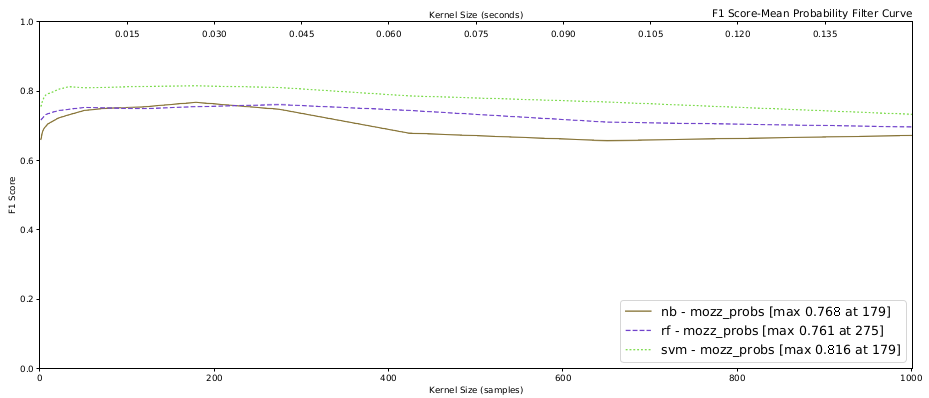
\includegraphics[width=0.9\textwidth]{meanfilt}
            \caption{F$_{1}$ scores as moving average filter kernel sizes are varied.}
            \label{fig:exp-postproc-filt}
        \end{figure}
        Kernel sizes, $K_{med}$ and $K_{mean}$, are tested over an exponential scale, decreasing from $1001$ samples (\SI{1/8}{\second}) to $3$ samples (\SI{0.375}{\milli\second}) through multiplying by powers of $0.65$. This reflects the expectation of smaller kernel sizes being more susceptible to noise and therefore producing more varied outputs. An example output graph is shown in figure \ref{fig:exp-postproc-filt}, where similar graphs have been generated for the median filter and for the metrics established previously. The best method and kernel size for filtering is chosen for each classifier. All the classifiers satisfy rejection and time resolution criteria, however, only the SVM reaches the minimum true negative rate required for specification I. All other metrics are unsatisfied, driving the need for more work on improving accuracy.

    \subsection{Rejection}
    \label{subsec:exp-postproc-rej}
        \begin{figure}[ht]
            \centering
            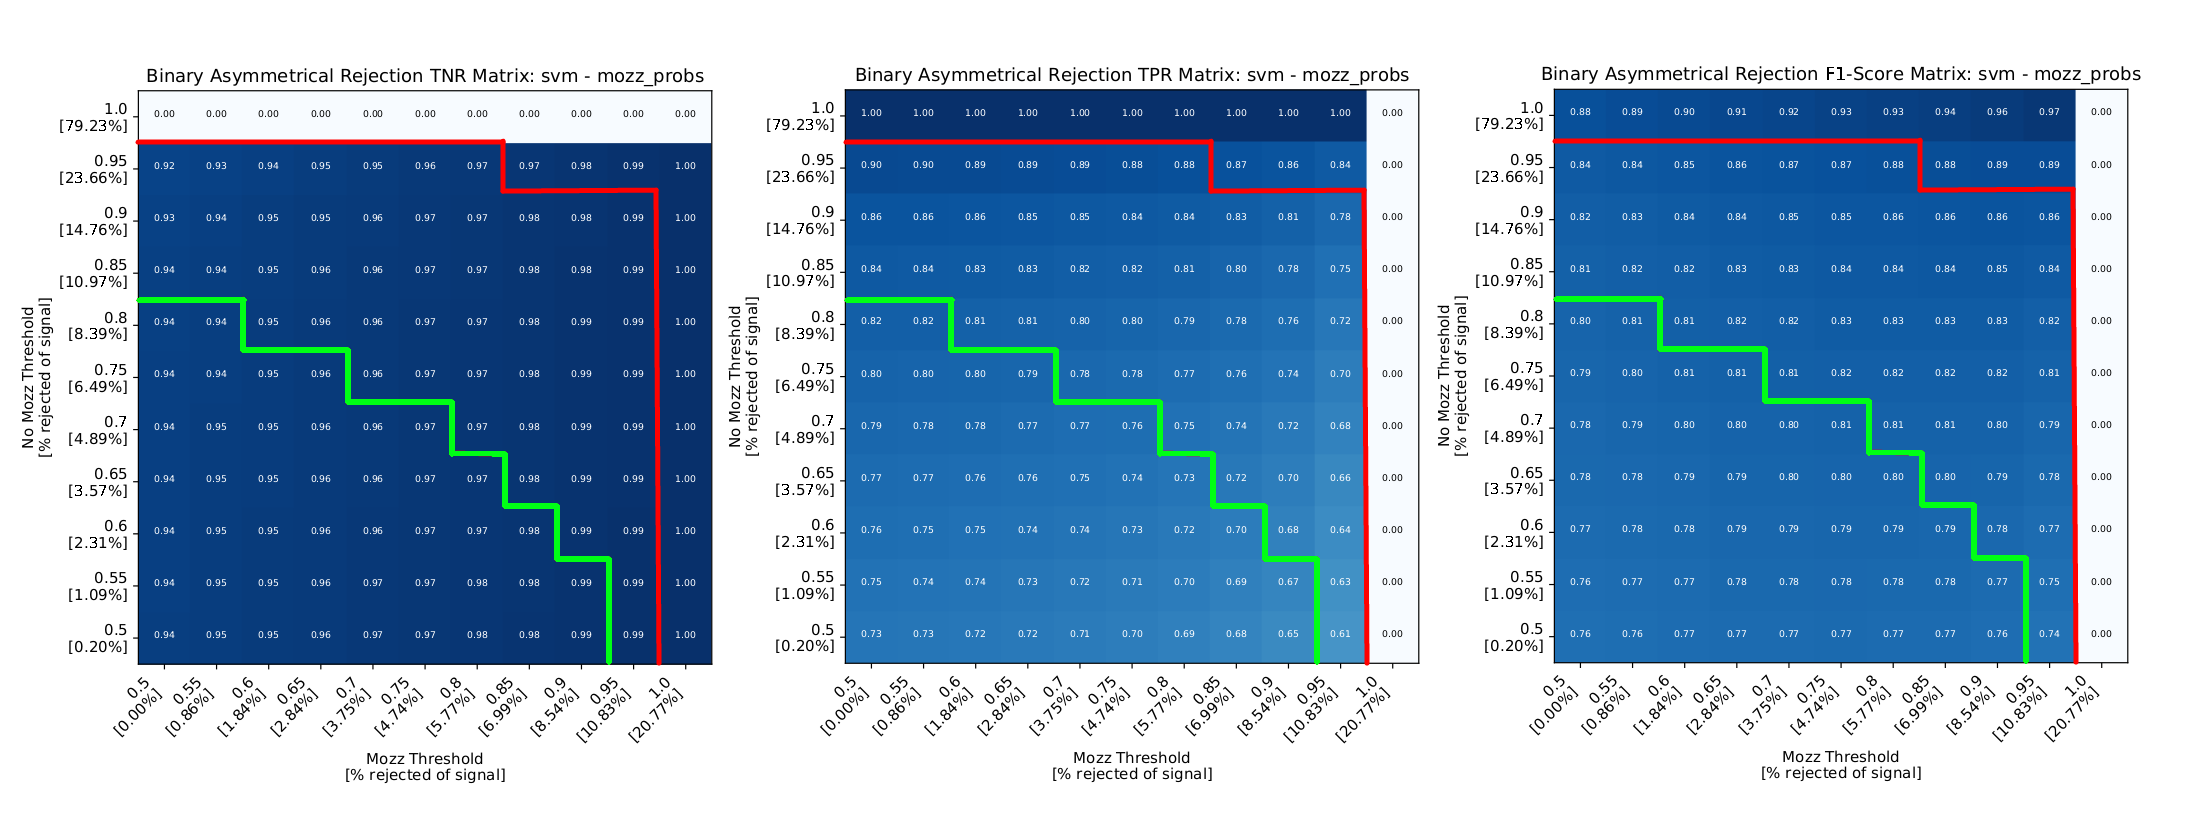
\includegraphics[width=\textwidth]{asymm_rej}
            \caption{From left to right shows a binary asymmetrical rejection matrix for the true negative rate, true positive rate and the $F_1$ score. On the $x$ axis are thresholds for the positive class, and on the $y$ are thresholds for the negative class. Under each threshold the percentage of the respective class rejected is shown.}
            \label{fig:exp-postproc-asymrej}
        \end{figure}
        Accuracy can also be increased through post-processing by rejecting predictions the classifier is less certain about. Metrics can be tuned at this stage due to the two degrees of freedom asymmetrical rejection offers. Figure \ref{fig:exp-postproc-asymrej} shows three metric-rejection grids for the SVM classifier, explained in section X, with bounds overlaid corresponding to the rejection criteria of the design specifications. The red bound indicates where rejection increases beyond $30\%$, and the green indicates where $10\%$ is surpassed. This means for specifications I and II, any pair of thresholds within the the red and green regions, respectively, can be chosen. This allows visual navigation of the asymmetrical performance-rejection space and enables straightforward hand-tuning of the classifier output. The chosen pairs are highlighted on each grid. Results indicate that although rejection alone improves performance, it is not enough to bring the true positive rates up to the specifications required.
    
    \subsection{Filtering and Rejection}
    \label{subsec:exp-postproc-filtrej}
        Thus far, rejection and smoothing have been applied in isolation. By applying them one after the other, further performance improvements can be made. However, the results depend on the order the post-processing is applied. If rejection is applied, followed by a smoothing filter over the probabilities, then the rejection becomes negligible, even at $30\%$. 
        \begin{figure}[ht]
            \centering
            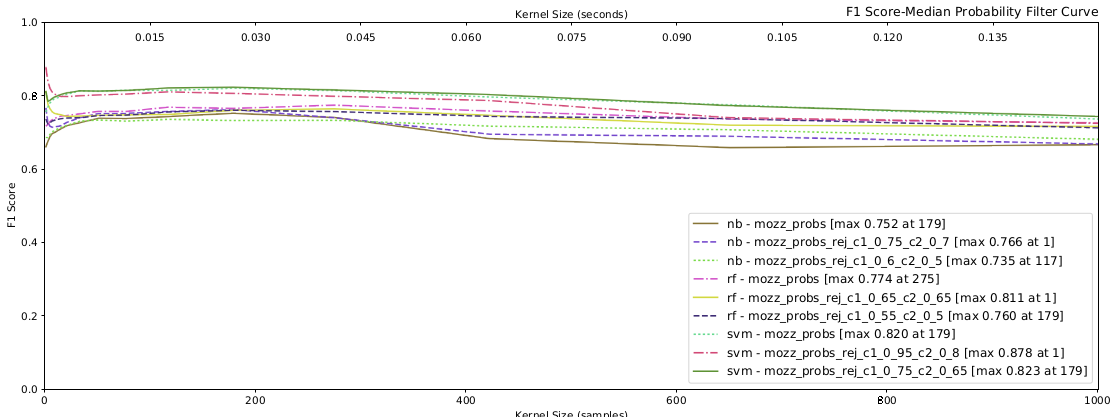
\includegraphics[width=\textwidth]{rej_filt}
            \caption{Median filtering applied to classifier outputs with varying degrees of rejection.}
            \label{fig:exp-postproc-rejfilt}
        \end{figure}
        Figure \ref{fig:exp-postproc-rejfilt} shows the sharp decline as the kernel size increases, followed by a gradual increase at the same rate as the results with no rejection. This indicates that these techniques are effective at removing noise in the predictions as the same results removed by rejecting probabilities are also smoothed out by a median filter. However, applied in a different order, results significantly improve. Repeating the filtering post-processing with the methods and thresholds determined in section \ref{subsec:exp-postproc-filt} and running through the same rejection-space analysis the results begin to approach the design requirements. The only classifier to fully meet specification is the naive Bayes classifier for specification I. The random forest comes close to meeting requirements but requirements are not quite satisfied. 